%% LyX 2.1.2 created this file.  For more info, see http://www.lyx.org/.
%% Do not edit unless you really know what you are doing.
\documentclass{sig-alternate}


% ------------- Packages Used --------------------------------------------------
% They help us to produce a better looking document ;-)
% ------------------------------------------------------------------------------

% Comment the following line before compiling the final version
%\synctex
\usepackage{multirow}

\usepackage{graphicx}
\usepackage{alltt}
\usepackage{relsize}
%\usepackage{xspace}
\usepackage{booktabs}
\usepackage{amsmath}
%\usepackage{multirow}
%\usepackage{array}
\usepackage{verbatim}
\usepackage[table]{xcolor}
\usepackage{caption}
\usepackage[labelformat=simple, labelsep=colon]{subcaption}{}
\captionsetup{compatibility=false}

%\usepackage[tight,footnotesize]{subfigure}

%\usepackage{capt-of}
%\usepackage{pifont}
\usepackage{amsfonts}
\usepackage{amssymb}
%\usepackage[latin1]{inputenc}
%\usepackage{times}
%\usepackage{colortbl}
%\usepackage{boxedminipage}
\usepackage{float}
%\usepackage{cite}
%\usepackage{fancyvrb}
%\usepackage{hyperref}
%\usepackage{balance}
\usepackage{url}
\usepackage{fancybox}%for \hypobox
\usepackage{listings}
\usepackage{array}
\usepackage{graphicx}
\usepackage{float}
%\usepackage{placeins}
\usepackage{multirow}
%\usepackage{blindtext}
%\usepackage{lipsum}
\usepackage{graphicx}
\usepackage{float}
%\usepackage{placeins}
\usepackage{multirow}
%\usepackage{caption} 

	
%\usepackage{subcaption}
%\usepackage{blindtext}
%\usepackage{lipsum}
\usepackage{graphicx}
\usepackage{amsmath}
\usepackage{booktabs}
\usepackage{framed}
\usepackage{multirow}% http://ctan.org/pkg/multirow
\usepackage{hhline}% http://ctan.org/pkg/hhline
\usepackage{amssymb}% http://ctan.org/pkg/amssymb
\usepackage{pifont}% http://ctan.org/pkg/pifont
\newcommand{\cmark}{\ding{51}}%
\newcommand{\xmark}{\ding{55}}%
%\usepackage{makecell}
%\usepackage{tablefootnote}

%\usepackage{textcomp}
%\usepackage{latexsym}
%\usepackage{amssymb}
%\usepackage{stmaryrd}
%\usepackage{euscript}
%\usepackage{wasysym}
%\usepackage{pifont}
%\usepackage{manfnt}
%\usepackage{undertilde}
%\usepackage{ifsym}
%\usepackage{tipa}
%\usepackage{txfonts}
%\usepackage{skak}
%\usepackage{skull}
%\usepackage{eurosym}
%\usepackage{yfonts}
%\usepackage{mathdots}
%\usepackage{trsym}
%\usepackage{upgreek}
%\usepackage{chemarr}
%\usepackage{accents}
%\usepackage{nicefrac}
%\usepackage{bm}


%\usepackage{pdfsync}

%   ACM Style
%\usepackage{lcsect}
% ------------------------------------------------------------------------------






% ------------ Color Definitions -----------------------------------------------
% Whatever colors we need
% ------------------------------------------------------------------------------
\definecolor{mygray}{rgb}{0.7,0.7,0.7}
% ------------------------------------------------------------------------------






% ---------- Special commands for annotating the paper's text ------------------
\let\mymarginpar\marginparm
\marginparwidth=1cm
\marginparsep=5pt
\newcommand{\todo}[1]{\textcolor{red}{\textbf{[[#1]]}}}
\def\TODO#1{\noindent\colorbox{yellow}{\bf \textcolor{red}{TODO: #1}}}
\newcommand{\hint}[1]{\textcolor{blue}{\textbf{#1}}}
\def\fig#1{Figure~\ref{#1}}
\def\tab#1{Table~\ref{#1}}
\def\eqn#1{Equation~\ref{#1}}
\def\sec#1{Section~\ref{#1}}

\pagenumbering{arabic}
\newcommand{\reviewer}[1]{\textcolor{DeepPink1}{{\it [Reviewer says: #1]}}}
\newcommand{\mei}[1]{\textcolor{red}{{\it [Mei says: #1]}}}
\newcommand{\ian}[1]{\textcolor{blue}{{\it [Ian says: #1]}}}
\newcommand{\nic}[1]{\textcolor{WildStrawberry}{{\it [Nico says: #1]}}}
\newcommand{\ahmed}[1]{\textcolor{green}{{\it [Ahmed says: #1]}}}
\newcommand{\myfoot}[1]{\footnote{\scriptsize #1}}
\newcommand{\myurl}[1]{\myfoot{\url{#1}}}
\newcommand{\Ra}{{$\Rightarrow$}}
\newcommand{\ra}{{$\rightarrow$}}
\newcommand{\La}{{$\Leftarrow$}}
\newcommand{\la}{{$\leftarrow$}}
\newcommand{\lra}{{$\leftrightarrow$}}
\newcommand{\LRa}{{$\Leftrightarrow$}}
%\newcommand{\todo}{\bram{todo}}

\newenvironment{myindentpar}[1]%
{\begin{list}{}%
         {\setlength{\leftmargin}{#1}}%
         \item[]%
}
{\end{list}}

% \AtBeginDocument{%
%    \renewcommand{\figurename}{Figure}%
%    \newcommand{\subfigureautorefname}{\figureautorefname}%for using subfig
% %   \renewcommand{\tablename}{TABLE}%
%    \renewcommand{\tablename}{Table}%
%    \renewcommand{\subsectionautorefname}{Section}%
%    \renewcommand{\sectionautorefname}{Section}%
% }

% Hypothesis box	
% ------------------------------------------------------------------------------	
\newcommand{\hypobox}[1]{\begin{center}%	
	\noindent\thicklines\setlength{\fboxsep}{7pt}%	
	\cornersize{0}\Ovalbox{\begin{minipage}{4.1in}%	
	\vspace{-0.1cm}
	\textit{#1}
	\vspace{-0.1cm}
	\end{minipage}} \end{center}}	
% ------------------------------------------------------------------------------




% ------------------------- SYMBOLS OF SELF NAMES OFTEN USED -------------------
\newcommand{\APACHE}{{\small APACHE}\xspace}
\newcommand{\BUGZILLA}{{\small BUGZILLA}\xspace}
\newcommand{\ECLIPSE}{{\small ECLIPSE}\xspace}
\newcommand{\ASPECTJ}{{\small ASPECTJ}\xspace}
\newcommand{\JDT}{{\small JDT}\xspace}
\newcommand{\GNU}{{\small GNU}\xspace}
\newcommand{\MOZILLA}{{\small MOZILLA}\xspace}
\newcommand{\THUNDERBIRD}{{\small THUNDERBIRD}\xspace}
\newcommand{\JAVA}{{\small Java}\xspace}
\newcommand{\GNOME}{{\small GNOME}\xspace}
\newcommand{\PG}{{\small PostgreSQL}\xspace}
\newcommand{\SIM}{{\small SimScan}\xspace}

% Anything else, e.g., \NAME{MICROSOFT}
\newcommand{\NAME}[1]{{\small #1}\xspace}
% ------------------------------------------------------------------------------




% ----------------------- Computer Science lol ---------------------------------
% Variable, function, and program names
% ------------------------------------------------------------------------------
\newcommand{\smalltt}[1]{\ifmmode{\mbox{\smaller\texttt{#1}}}\else{\smaller\tt #1}\fi}
\newcommand{\code}[1]{\smalltt{#1}}
\newcommand{\var}[1]{\code{#1}}
\newcommand{\func}[1]{\code{#1}}
\newcommand{\proc}[1]{\code{#1}}
\newcommand{\prog}[1]{\code{#1}}
\newcommand{\type}[1]{\code{#1}}
\newcommand{\progpt}[1]{\code{#1}}

\newcommand{\mypar}[1]{\vspace{.1cm}\noindent \textbf{#1}}
\newcommand{\myxpar}[1]{\vspace{.1cm}\noindent \textbf{#1}\newline}
% ------------------------------------------------------------------------------





% ----------- Things to remember -----------------------------------------------
\newenvironment{mynote}%
{ \medskip
  \noindent
  \let\emph=\textbf
  \begin{boxedminipage}{\columnwidth}\em}%
{ \end{boxedminipage}}
% ------------------------------------------------------------------------------






% -------------------- Use bars ------------------------------------------------
% These macros are for advanced presentation of results by shaded bars only!
% © Tom Zimmermann, 2008
% ------------------------------------------------------------------------------
\newdimen\qdx
\newdimen\qda
\newdimen\qdb
\def\rrrr#1#2#3#4{\newdimen\qd\qd=#4 % length of bar for 1.0
\qdx=\qd\multiply\qdx by 5\divide\qdx by 4
\qda=\qd
\qdb=\qd
\multiply\qda by #1\divide\qda by #3\multiply\qdb by #2\divide\qdb by #3\advance\qdb by -\qda
    \leavevmode\hbox to \qdx{\hfil\vbox{%
    \hbox{\vrule\vbox{\hrule\hbox to 1\qd
            {\vrule depth0pt height0.7ex width \qda\color{mygray}%
 \vrule depth0pt height0.7ex width \qdb\hfill}\hrule}\vrule}
    }\hfil}}
\def\rrr#1#2#3{\rrrr{#1}{#2}{#3}{0.8cm}}
% -------------------------------------------------------------------------






% ------------ Graphics Hacks --------------------------------------------------
% Use these settings if Figures tend to get their one separate pages
% ------------------------------------------------------------------------------
% \renewcommand{\topfraction}{0.85}
% \renewcommand{\textfraction}{0.1}
% \renewcommand{\floatpagefraction}{0.75}
% ------------------------------------------------------------------------------





% ------------------ Biblio Hack -----------------------------------------------
% Use these settings if the References take too much space
% ------------------------------------------------------------------------------
\let\oldthebibliography=\thebibliography
  \let\endoldthebibliography=\endthebibliography
  \renewenvironment{thebibliography}[1]{%
%	\vspace{-0.3cm}
    \begin{oldthebibliography}{#1}%
%	\vspace{-0.2cm}
       \setlength{\parskip}{0ex}%
       \setlength{\itemsep}{0ex}%
%	\bibfont
  }%
  {%
    \end{oldthebibliography}%
  }
% ------------------------------------------------------------------------------





% -------------- Floats Redefined ----------------------------------------------
% Use these settings to change the whitespace between floats and text
% ------------------------------------------------------------------------------

% \setlength\dblfloatsep{1pt}
% \setlength\floatsep{1pt}
% \setlength\textfloatsep{5pt}
% \setlength\dbltextfloatsep{5pt}

% \renewcommand\floatpagefraction{.9}
% \renewcommand\topfraction{.9}
% \renewcommand\bottomfraction{.9}
% \renewcommand\textfraction{.1}
% \setcounter{totalnumber}{50}
% \setcounter{topnumber}{50}
% \setcounter{bottomnumber}{50}
% ------------------------------------------------------------------------------
\makeatletter

%%%%%%%%%%%%%%%%%%%%%%%%%%%%%% LyX specific LaTeX commands.
%% Because html converters don't know tabularnewline
\providecommand{\tabularnewline}{\\}

\begin{document}
	
	
	
	\title{An Empirical Study On Leveraging Logs During Bug Fixes}
	
	
	
	\numberofauthors{1}
	
	
	\author{\alignauthor Suhas Kabinna, Weiyi Shang, Ahmed E. Hassan\\
		\affaddr{School of Computing}\\
		\affaddr{Queen's University}\\
		\affaddr{Kingston, Ontario, Canada K7L 2N8}\\
		\email{\{kabinna, swy, ahmed\}@queensu.ca}\\
	}
	


%\additionalauthors{Additional authors: John Smith (The Th{\o}rv{\"a}ld Group, email:
%\texttt{jsmith@affiliation.org}) and Julius P.~Kumquat (The Kumquat
%Consortium, email: \texttt{jpkumquat@consortium.net})}


\date{30 July 1999}
\maketitle
\begin{abstract}
	\indent Logging is a practice used by software developers to record and convey
	information during the execution of a system. Logs can be used to
	output the behavior of the system when running, to monitor the choke
	points of a system, and to help in debugging the system.
	
	Though much research has been done on the analysis of logs, most of
	the studies looked at either characterizing logs based on their usage
	or how to improve logs so they are more meaningful. But, there has
	been no study so far which looks into how effective logs are in the
	software development process and especially in debugging. 
	
	To answer this question in our paper we first try to find co-relation
	between log updates and bug fixes. This is an intuitive step, because
	when developers fix bugs they update the logs associated with the
	bug or add new logs to help them fix bugs. We verify this claim on
	3 large scale systems like Hadoop, HDFS and Qpid from the Apace Foundation.
	We then find the types of changes developers make to logging statements
	during bug fixes. Finally, we look at how long it takes for bugs to get fixed,
	the number of developers involved in the fix and the comments associated
	with the fixes, all with respect to bugs without logging changes.\\
	\indent We find that in all projects logging actually helps in the debugging
	process and three factors - time, developers and comments - are lesser
	when bugs have log churn associated with them. This demonstrates the
	importance logs play in bug fixes and motivates developers to log
	more.
\end{abstract}

% A category with the (minimum) three required fields; A category including the fourth, optional field follows...


%\category{H.4}{Information Systems Applications}{Miscellaneous}

%Full ACM categories cannot be yet represented in LyX without resorting to ELT
%\category{D.2.8}{Software Engineering}{Metrics}[complexity measures, performance measures]


%\terms{}{Theory}


%\keywords{}{ACM proceedings, \LaTeX{}, text tagging}


\section{Introduction}

Platform software provides an infrastructure for a variety of applications that run on top of it. Platform software often relies on logs to monitor the applications that run over it. Such logs are generated through simple \textsl{printf} statements or through the use of logging libraries such as `Log4j', `Slf4j', and `JCL'. Each logging statement contains a static textual part that gives information about the context,  a variable part that contains knowledge about the events, and a logging verbosity level that indicates when the log should be output. An example of a log is shown below where \emph{info} is the logging level, \emph{Connected to} is the event and the variable \emph{host} contains the information about the logged event. 

\hypobox{ \hspace{25pt} LOG.info( ``Connected to " + host);}

 In our paper we use `log' to refer to the logging statements in the source code, and use `output log' to refer to the logs generated during system execution. We use the term `bug fix' to refer to the commits made to fix a bug, and `non-bug fix' refers to commits made during improvements, tests, new features and other tasks.
 
Research has shown that logs are used by developers extensively during the development of software systems~\cite{Characterizinglogs}. Logs are leveraged for anomaly detection~\cite{XUanomalies,ConsoleLogs,Marksyer}, system monitoring~\cite{Bitperformance}, capacity planning~\cite{IanWCRE} and large-scale system testing~\cite{markTesting}. The valuable information in logs has created a new market for log maintenance platforms such as Splunk~\cite{Bitperformance}, XpoLog~\cite{Xpolog}, and Logstash~\cite{Logstash}, which assist developers in analyzing logs.

Logs are extensively used to help developers fix bugs in platform software. For example, in the JIRA issue HBASE-3403\footnote{https://issues.apache.org/jira/browse/HBASE-3403}, a bug was reported when a region is orphaned when system failure occurs during a split. Developers leveraged logs to identify the point of failure. After fixing the bug, the logs were updated to prevent similar bugs from re-occurring. A recent study shows that changes to logs have a strong relationship with code quality~\cite{EMSEIAN}. However, there exists no large scale study that investigate how logs are changed during bug fixes.  This information is necessary as previous research shows that 16-32\% of logs changes are made during field debugging~\cite{EMSEIAN}, but how these changes are made is not understood. 


In this paper, we perform an empirical study on the changes that occur to logs during bug fixes in three open source platform software, i.e., \emph{Hadoop}, \emph{HBase} and \emph{Qpid}. In particular, we sought to answer the following research questions. 

\begin{description}
\item[\textbf{RQ1:}]\textbf{Are logs changed more often during bug fixes?} 

We find that logs are changed more often during bug fixes than non-bug fixes. In particular, we find that adding and modifying logs occurs more often in bug fixes than non-bug fixes (statistically significant with non-trivial effect size). We identified four types of modifications to logs, including \emph{modification to logging level}, \emph{modification to logging text}, \emph{modification of logged variable} and \emph{relocation of log}. We find that \emph{modification to logging text}, \emph{modification of logged variable} and \emph{relocation of log} occur more often in bug fixes than non-bug fixes (statistically significantly more with medium to high effect sizes). 



\item[\textbf{RQ2:}]\textbf{Is there relation between log change and resolution time of bug fixes?}

We find that bug fixes with log churn have higher total code churn than bug fixes with no log churn. After normalizing the code churn, bug fixes with log churn take less time to get resolved, involve fewer developers and have less discussions during the bug fixing process. This means that given two metrics of similar complexity the one with log churn is more likely to be resolved faster and involve fewer developers and less discussion. 



\item[\textbf{RQ3:}]\textbf{Can log churn metrics explain the resolution time of bugs?}

Using log churn metrics (e.g., new logs added, deleted logs) and traditional metrics (i.e., \# comments and \# developers) we trained regression models for the resolution time of bug fixes. We find that log churn metrics are statistically significant in the models and have negative impact on resolution time. This suggests there is a relation between log churn metrics and resolution time of bugs. The relation shows that log churn has impact on resolution time which should be studied further. 

\end{description}


The rest of this paper is organized as follows. Section~\ref{sec:Methodology} presents our methodology for extracting data for our study. Section~\ref{sec:Study} presents our case study and the answers to our three research questions. Section~\ref{sec:Related} describes the prior research that is related to our work. Section~\ref{sec:Limit}  discusses the threats to validity. Finally, Section~\ref{sec:Conclusion} concludes the paper.



\section{Related Work}


In this section, we present the prior research that performs log analysis on large software systems and empirical studies on logs. 


\subsection{Log Analysis}

% The purpose of this section is to highlight the research that shows
%logs are used in debugging process. This is related to our work because
%(1) we show that logs are used in all the processes of a software
%life cycle, (2) how logs are useful in the improving the quality of
%the software. 
%\ian{some names are textsl, some are not. I think just keep the name as regular font and put et al. as italic, sometimes you miss the . in et al. and you should put dollar signs before and after the .}
Prior work leverage logs for testing and detecting anomalies in large scale systems. Shang\textsl{ et al$.$}~\cite{IanContextinformation} propose an approach to leverage logs in verifying the deployment of Big Data Analytic applications. Their approach analyzes logs in order to find differences between running in a small testing environment and a large field environment. Lou \textsl{et al}$.$~\cite{JGLouMining} propose an approach to use the variable values printed in logs to detect anomalies in large systems. Based on the variable values in logs, their approach creates invariants (e.g., equations). Any new logs that violates the invariant are considered to be a sign of anomalies. Fu \textsl{et al}$ . $~\cite{QFuanomaly} built a Finite State Automaton (FSA) using unstructured logs and to detect performance bugs in distributed systems. 

\indent Xu \textsl{et al}$ . $~\cite{ConsoleLogs} link logs to logs in source code to recover the text and and the variable parts of output logs. They applied Principal Component Analysis (PCA) to detect system anomalies. Tan \textsl{et al}$ . $~\cite{TanSalsa} propose a tool named SALSA, which constructs state-machines from logs. The state-machines are further used to detect anomalies in distributed computing platforms. Jiang \textsl{et al}$ . $~\cite{Jiang:2009:UCP:1525908.1525912} study the leverage of logs in troubleshooting issues from storage systems. They find that logs assist in a faster resolution of issues in storage systems. Beschastnikh \textsl{et al}$ . $~\cite{Beschastnikh:2011:LEI:2025113.2025151} designed automated tools that infers execution models from logs. These models can be used by developers to understand the behaviours of concurrent systems. Moreover, the models also assist in verifying the correctness of the system and fixing bugs.

To assist in fixing bugs using logs, Yuan \emph{et al$.$}~\cite{Yuan:2010:SED:1736020.1736038} propose an approach to automatically infer the failure scenarios when a log is printed during a failed run of a system.


Jiang \textsl{et al$ . $}~\cite{Jiang:2008:AAA:1400155.1400158,JiangICSM2008,JiangICSM20092,Jiang:2010:ICS:1850000.1850068} proposed log analysis approaches to assist in automatically verifying results from load tests. Their log analysis approaches first automatically abstract logs into system events~\cite{Jiang:2008:AAA:1400155.1400158}. Based on the such events, they identified both functional anomalies~\cite{JiangICSM2008} and performance degradations~\cite{JiangICSM20092} in load test results. In addition, they proposed an approach that leverage logs to reduce the load test that are performed in user environment~\cite{Jiang:2010:ICS:1850000.1850068}.

The extensive prior research of log analysis motivate our paper to study how logs are leveraged during bug fixes. As a first step, we study the changes to log during bug fixes. Our findings show that logs are change more during bug fixes than other types of code changes. The changes to logs have a relationship with a faster resolution of bugs with fewer people and less discussion.



% This is similar to our work
%because, we also use source code parsing in finding the logs. But
%instead of trying to build structured logs we try to classify them
%using levenshtein distances.

% Similar work has been done to show how mining execution logs in large systems can help  detect anomalies and ensure good load tests  \textsl{Malik et al}\cite{Automatic}. This paper  \textsl{Lou et al}\cite{JGLouMining} discuss how invariants, mined from console logs can help to detect anomalies in large systems. \textsl{Fu et al}\cite{QFuanomaly} shows analysis of unstructured logs helps in detecting performance bugs in Distributed systems. Tools have also been developed to diagnose failures by mining execution logs \textsl{Tan et al}\cite{TanSalsa}. 

%Work has been done on mining execution logs in Big Data Analytic (BDA)
%applications to find difference in behavior of the system, when tests
%are run on small testing data and actual real world data \cite{IanContextinformation}.
%Similar work has been done to show how mining execution logs in large
%systems can help in detecting anomalies and ensure good load tests
%\cite{Automatic}. In the paper execution logs are mined and event
%pair are formed. By finding patterns in these event pairs dominant
%behavior of the system is identified. Any event which does not follow
%this is tagged as anomaly and can be reported to the developers. These
%papers show that logs are not used only for the purpose of debugging
%but can assist a developer in a variety of tasks. 
%
%Research has been to detect anomalies by invariant mining\cite{JGLouMining}.
%This paper focuses on constructing structured logs from console logs.
%After construction and grouping of log messages, invariants are mined.
%Any log which violates a invariant is considered to be an anomaly.
%Unstructured log analysis has shown to be useful in detecting in even
%Distributed Systems Several \cite{QFuanomaly}. In the paper a finite
%state automaton is built and trained to automatically detect performance
%bugs in the system. These papers consider print messages and other
%unstructured logs to extract information. Then they cluster or categorize
%the logging messages into groups and logs which fall into this cluster
%are treated as anomalies. Tools have also been developed to analyze
%system logs to obtain state-machine view, control and data flow models
%and other related statistics. SALSA\cite{TanSalsa} helps in deriving
%failure diagnosis techniques and visualization for different workloads
%in Hadoop project by mining execution logs. In our study, though we
%use the same system software (Hadoop),we try to understand how logs
%can be useful in debugging and not on trying to find the bug itself. 



\subsection{Empirical studies on logs}

%In this section we try and find out how developers log. Is it done
%manually or do developers use established logging libraries. From
%our work on studying logging libraries in the Apache foundation we
%know that Slf4j, Log4j and Jakarta common logging are the most used
%libraries for logging. This helps us to find the logs
%in our case studies. Additionally there are many tools which help
%developers in logging \cite{Yuan}. The authors conduct a manual analysis and find that logs help in understanding the control and data flow in bug fixes but do not contain all the information to conclusively answer why the bug occurs. The paper addresses this issue through a tool called 'Log Enhancer' to enhance existing logs by providing additional details in the logs. This was tested with earlier version
%of the software and it was observed that 95\% of logs added by the
%tool were added by developer\textquoteright s overtime. This paper
%highlighted that do not log all the details in the first deployment
%and modify the logs in later revisions. This conforms to our findings
%as well, as we found that developers modify logs during debugging
%than other software process. 

Prior research performs an empirical study on the characteristics of logs. Yuan \textsl{et al}$ . $~\cite{Characterizinglogs} studies the logging characteristics in four open source systems. They find that over 33\% of all log changes are after thoughts and logs are changed 1.8 times more than entire code. Fu \textsl{et al$.$}~\cite{Fu1} performed an empirical study on where developer put logs. They find that logs are used for assertion checks, return value checks, exceptions, logic-branching and observing key points. The results of the analysis were evaluated by professionals from the industry and F-score of over 95\% was achieved. 


Shang \textsl{et al$ . $}~\cite{IanGap} signify the fact that there is gap between operators and developers of software systems, especially in the leverage of logs. They performed an empirical study on the evolution both static logs and logs outputted during run time~\cite{EMSEIAN,PaperIanCIIII}. They find that logs are co-evolving with the software systems. However, logs are often modified by developers without considering the needs of operators. Furthermore, Shang\textsl{ et al$ . $}~\cite{IanIcesm} find that understanding logs is challenging. They examine user mailing lists from three large open-source projects and find that users of these systems have various issues in understanding logs outputted by the system. Shang\textsl{ et al$ . $} propose to leverage different types of development knowledge, such as issue reports, to assist in understanding logs. 

Prior research by Yuan\textsl{ et al$ . $}~\cite{Yuan} shows that logs need to be improved by providing additional information. Their tool named \emph{Log Enhancer} can automatically provide additional control and data flow parameters in the logs thereby improving the output logs. Log Advisor is another tool by Zhu \emph{et al$.$}~\cite{zhu2015learning} which helps in logging by learning where developers log through existing logging instances. 

The most related prior research by Shang \emph{et al$.$}~\cite{EMSEIAN} empirically study the relationship of logging practice and code quality. Their manual analysis sheds light on the fact that some logs are changed due to field debugging. They also show that there is a strong relationship between logging practice and code quality. Our paper focused on understanding how logs are changed during bug fixes. Our results show that logs are leveraged extensively during bug fixes and may assist in the resolution of bugs. 


\section{Methodology}
In this section, we describe our methodology for preparing the data to answer our research questions.

The aim of this paper is to understand how logs are changed during bug fixes and the relationship between bug resolution time and log changes. We conduct a case study on three open source platform software, i.e., \textsl{Hadoop, HBase} and \textsl{Qpid}. All three platform softwares have extensive logging in their source code. Table~\ref{tba:Overview} highlights the overview of the three platform software.

\begin{table}[t]
	\protect\caption{An overview of the platform software}
	\label{tba:Overview}
	\centering{}%
	\begin{tabular}{|>{\centering}p{.15\textwidth}|>{\centering}p{.1\textwidth}|>{\centering}p{.1\textwidth}|>{\centering}p{.1\textwidth}|>{\centering}p{.1\textwidth}|>{\centering}p{.1\textwidth}|>{\centering}p{.1\textwidth}|}
		\hline 
		\multirow{2}{*}{Projects} & \multicolumn{2}{c|}{Hadoop} & \multicolumn{2}{c|}{HBase} & \multicolumn{2}{c|}{Qpid}\tabularnewline
		\cline{2-7} 
		& Bug fixing  & Non-bug fixing & Bug fixing  & Non-bug fixing & Bug fixing  & Non-bug fixing \tabularnewline
		\hline 
		Total \# of commits & 1,808 & 1,809 & 1924 & 1463 & 953 & 875\tabularnewline
		
		
		 & (49.9 \%) & (50.1 \%) & (56.8 \%) & (43.2 \%) & (52.1 \%) & (47.9 \%) \tabularnewline
		\hline 
		 
		Code churn (LOC) & 246 K & 1.8 M & 653 K & 1.5 M &  106 k & 597 K\tabularnewline
		\hline 
		Log churn (LOC) & 3,536 & 16,980 & 4,672 & 10,335 & 972 & 4,953\tabularnewline
		\hline 
		\% of Commits with log churn & 24.0 \% (433) &  46.2 \% (656) & 36.2 \% (648) & 42.1 \% (616) & 22.1 \% (211) & 32.8 \% (287) \tabularnewline
		\hline		
	\end{tabular}
\end{table}



{\textbf{Hadoop}\footnote[1]{http://hadoop.apache.org/}}: \emph{Hadoop} is an open source platform for distributed storage and processing of big data on computer clusters. \emph{Hadoop} uses the MapReduce data-processing paradigm. The logging characteristics of \emph{Hadoop} have been extensively studied in prior research~\cite{JGLouMining,EMSEIAN,ConsoleLogs}. We study the changes to logs from \emph{Hadoop} releases $0.16.0$ to $2.0$.


{\textbf{HBase}\footnote[2]{http://hbase.apache.org/}}: \emph{HBase} is a distributed, scalable, big data software, which uses \emph{Hadoop} file-systems. We study the changes to logs in \emph{HBase} from release $0.10$ to $0.98.2.RC0$. This covers more than four years of development in \emph{HBase} from 2010 to 2014.

{\textbf{Qpid}\footnote[3]{https://qpid.apache.org}}: \emph{Qpid} is an open source messaging platform that implements an Advanced Message Queuing Protocol (AMQP). We study \emph{Qpid} release $0.10$ to release $0.30$ that are from 2011 till 2014.


Figure~\ref{tba:Overview} shows a general overview of our approach, which consists of four steps: (1) We mine the git repository of each studied system to extract all commits, and identify bug-fixing commits (bug fixes) non-bug-fixing commits (non-bug fixes). (2) We identify log changes in both bug fixes and non-bug fixes. (3) We categorize the log changes into three types, \textsl{`New logs', `Modified Logs'} and \textsl{`Deleted logs'}. (4) We calculate churn metrics for each type and use a statistical tool R~\cite{ihaka1996r}, to perform experiments on the data to answer our research questions.  In the reminder of this section we describe the first three steps.

%We used Apache software versioning system, SVN to collect the commit
%history for all the projects in our case study. We used JIRA to collect
%the buggy reports for all the projects in our case study. We extracted
%the reports in XML format for parsing convenience. 


\subsection{Study Approach}

In this section, we present the first three steps of our study approach. 
%We use Git to study the evolution of Java source code in the three subject systems. 
%%similar to C-REX ~\cite{HassanPHD} and J-REX ~\cite{WCSEIan}. 
%We extract the changes in each commit and use this data to calculate the metrics to answer our research questions.
\begin{figure}[t]
	\centering
	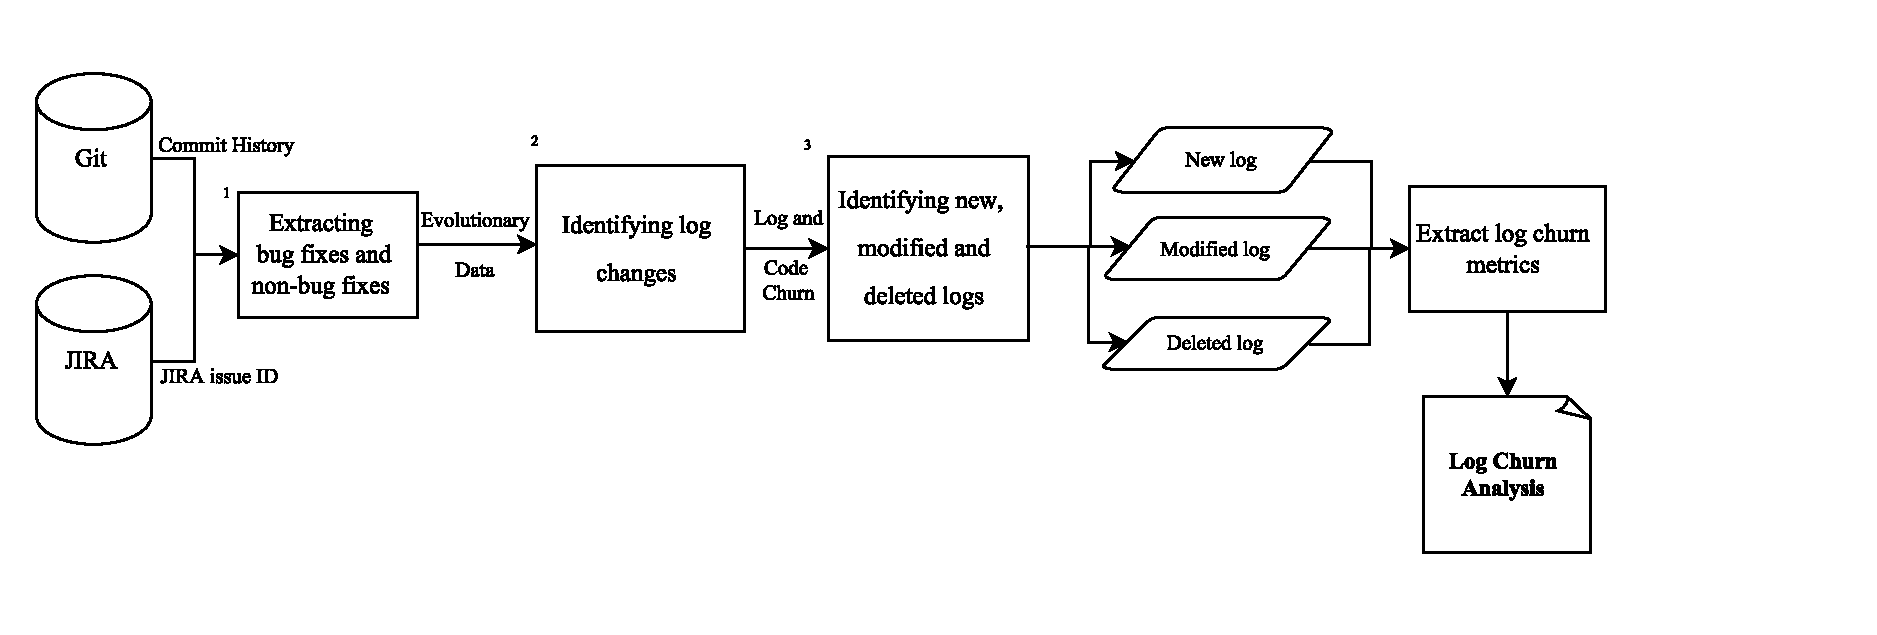
\includegraphics[scale=0.45]{MethdologyICESEM}
	\caption{Overview of our case study approach }
	\label{fig:MethodologyICSME}
\end{figure}

\subsubsection{Extracting bug fixes and non-bug fixes}

The first step in our approach is to extract commits that are associated with bug fixes and the ones that are not associated with bug fixes. First, we extract a list of all commits from the git repository of each project. To avoid the branching and merging commits, we enable the `no-merges' option in the git \textsl{log} command. This flattens all the changes that are made to file in different branches and excludes the final merge between branch and trunk. We also filter out the changes to non-Java files or the test files from the commits. 

Next, we extract a list of all the JIRA issues that have the type \emph{bug}. Developers often mention the JIRA issue ID's in the commit messages. We search JIRA issue IDs in the commit messages to identify all the bug fixes. We exclude commits that do not contain any JIRA ID since we cannot identify if the commit is a bug fix or not. 

\subsubsection{Identifying log changes}

To identify the log changes in the datasets, we first manually explore logs in the source code. Some logs are specific to a particular project. For example, a log from Qpid invokes `QPID\_LOG' to print logs as follows: 
\hypobox{QPID\_LOG(error, ``Rdma: Cannot accept new connection (Rdma exception):
	'' + e.what());
	}

Some logs leverage logging libraries to print logs. For example, \textsl{Log4j}\footnote{http://logging.apache.org/log4j/1.2/} is used widely in \emph{Hadoop} and \emph{HBase}. In both projects, logs have a method invocation `LOG', followed by a logging level. The following log uses \textsl{Log4j}:
\hypobox{ LOG.debug(``public AsymptoticTestCase(String''+ name +``) called'')}

Using regular expressions to match these logs, we automate the process of finding all the logs in the studied projects.


\subsubsection{Identifying new, modified and deleted logs}

Since git \textsl{diff} does not track modification to the code, modifications to a log is shown as a deletion followed by an addition. To track these added and deleted logs we used Levenshtein ratio~\cite{Levenshtein2}. For every pair of added or deleted logs in a commit, we compare the text in parenthesis after removing the logging method (e.g, LOG ) and the log level (e.g, info). We calculate the Levenshtein ratio between the added and deleted log similar to prior research~\cite{levenshteinratio}. We consider a pair of added and deleted logs as a log modification if they have a Levenshtein ratio of 0.6 or higher. For example, the logs shown below have Levenshtein ratio of 0.86. Hence such a pair of added and deleted logs are categorized as a log modification.  
\hypobox{+      LOG.debug(``Call: " +method.getName()+`` took "+ callTime + ``ms");\\ 
	-        LOG.debug(``Call: " +method.getName()+ `` " + callTime);} 

If an added log has a Levenshtein ratio higher than 0.6 with more than one deleted log, we consider the pair of added and deleted logs with the highest Levenshtein ratio as a log modification. After identifying all log modifications, we identify three types of log changes in a commit namely `new logs', `deleted logs' and `modified logs'.



\section{Study Results}

In this section we present our study results by answering our research questions. For each question, we discuss the motivation behind it, the approach to answering it and finally the results obtained.

\begin{table*}
	\caption{Summary of metrics}
	\label{tab:bla}
	\centering{}%
	\begin{tabular}{|c|c|c|c|c|c|c|c|}
		\hline 
		\multirow{2}{*}{Projects} & \multirow{2}{*}{Metrics} & \multicolumn{3}{c|}{Non-Bug fixing Commits} & \multicolumn{3}{c|}{Non-Bug fixing Commits}\tabularnewline
		\cline{3-8} 
		&  & Min Value & Max Value & Mean Value & Min Value & Max Value & Mean Value\tabularnewline
		\hline 
		\multirow{3}{*}{Hadoop} & New Logs & 0 & 184 & 0.245 & 0 & 197 & 0.533\tabularnewline
		\cline{2-8} 
		& Removed Logs & 0 & 33 & 0.093 & 0 & 143 & 0.175\tabularnewline
		\cline{2-8} 
		& Modified Logs & 0 & 67 & 0.124 & 0 & 83 & 0.227\tabularnewline
		\hline 
		\multirow{3}{*}{Hbase} & New Logs & 0 & 211 & 0.309 & 0 & 534 & 0.718\tabularnewline
		\cline{2-8} 
		& Removed Logs & 0 & 49 & 0.147 & 0 & 233 & 0.281\tabularnewline
		\cline{2-8} 
		& Modified Logs & 0 & 71 & 0.209 & 0 & 187 & 0.271\tabularnewline
		\hline 
		\multirow{3}{*}{Qpid} & New Logs & 0 & 87 & 0.116 & 0 & 477 & 0.796\tabularnewline
		\cline{2-8} 
		& Removed Logs & 0 & 23 & 0.046 & 0 & 97 & 0.270\tabularnewline
		\cline{2-8} 
		& Modified Logs & 0 & 72 & 0.084 & 0 & 125 & 0.343\tabularnewline
		\hline 
	\end{tabular}
\end{table*}



\begin{table*}[t]
	\caption{P values and Effect Size of for comparison	. A positive effect size means bug fixing commits are larger. P-values are bold if it is less than 0.05.}
	\label{tab:logchange}
	\centering{}%
	\begin{tabular}{|>{\centering}m{4.1cm}|>{\centering}m{1.5cm}|c|>{\centering}p{1.5cm}|c|>{\centering}p{1.5cm}|c|}
		\hline 
		Projects & \multicolumn{2}{c|}{Hadoop} & \multicolumn{2}{c|}{Hbase} & \multicolumn{2}{c|}{Qpid}\tabularnewline
		\hline 
		Metrics & P-Values & Effect Size & P-Values & Effect Size & P-Values & Effect Size\tabularnewline
		\hline 
		Modified Log Churn  & \textbf{2.88e-4} & 0.167(small) & \textbf{0.0353} & 0.0886 & \textbf{0.0281} & 0.329(small)\tabularnewline
		\hline 
		New Log Churn & \textbf{0.00202} & 0.0078 & \textbf{0.00353} & 0.134 & \textbf{0.0032} & 0.234(small)\tabularnewline
		\hline 
		Deleted Log Churn & 0.087 & -0.0455 & \textbf{0.00489} & 0.120 & \textbf{0.00952} & 0.042\tabularnewline
		\hline 
	\end{tabular}
	
\end{table*}



\subsection*{\textbf{RQ1: Are logs leveraged more during bug fixes? }}


\subsubsection*{\textbf{Motivation}}

Prior research has shown that logs are used during bug fixing~\cite{EMSEIAN}. During debugging, developers update log statements, to gain more run-time information of the systems and ensure that future occurrences of a similar bug can be resolved easily with the updated information. 
However, to the best of our knowledge, there exists no large scale empirical study to show how extensively logs are leveraged during bug fixes. Moreover, little is known about how bugs are leveraged during bug fixes. 


% But, this is not
%the only reason for using logging in a system. So in our first research
%question we try to address this issue. Answering this questions helps
%us understand where developers log more.


\subsubsection*{\textbf{Approach}}

%Its intuitive that logs are generally modified when bugs are fixed.
%This is because prior research has already proved that a module
%that has been modified continually, has higher chance
%of having bugs than modules which have not been modified \cite{Khosh}.
%So,
We try to find if there is a difference between bug fixing and non-bug fixing commits with respect to log churn. To do this, we used the data sets obtained in previous section i.e modified, new and removed logs, and we calculated code churn for each data set. We used the total code churn of a revision to control the other metrics. The 3 new metrics are:
\begin{equation}
Modified\ log\ churn\ ratio = \frac{\#\ modified\ log}{total\ code\ churn } 
\label{eq1}
\end{equation}
\begin{equation}
New\ log\ churn\ ratio = \frac{\#\ new\ log}{total\ code\ churn } 
\label{eq2}
\end{equation}
\begin{equation}
Removed\ log\ churn\ ratio = \frac{\#\ removed\ log\ churn}{total\ code\ churn }
\label{eq3} 
\end{equation}

To determine whether there is a statistically significant difference for these metrics, in bug-fixing and non-bug-fixing commits, we perform the \textsl{MannWhitney U test} (Wilcoxon rank-sum test)~\cite{gehan1965generalized}. We choose {\em MannWhitney U test} because we our metrics are highly skewed (shown in table~\ref{tab:bla}) and as it is a non-parametric test, which does not have any assumptions about the distribution of the sample population. A p-value of \ensuremath{\le} 0.05 means that the difference between the two data sets is statistically significant and we may reject the null hypothesis (i.e., there is no statistically significant difference of our metrics in in bug-fixing and non-bug-fixing commits). By rejecting the null hypothesis, we can accept the alternative hypothesis, which tells us there is statistically significantly difference of our metrics in bug-fixing and non-bug-fixing commits.

%and if we use standard T-test the
%resulting p-value will be wrong. {\em Wilcoxon test} is a non-parametric
%test, meaning the distribution of the population does not factor into
%the results.

We also use {\em effect sizes} to measure how big is the difference of our metrics ($modified\ log\ churn\ ratio$, $new\ log\ churn\ ratio$, and $removed\ log\ churn\ ratio$) between the bug fixing and non-bug-fixing commits. Unlike {\em MannWhitney U test}, which only tells us whether the difference between the two distributions are statistically significant, effect sizes quantify the difference between two distributions. Researchers have shown that reporting only the statistical significance may lead to erroneous results  (i.e., if the sample size is very large, p-value can be small even if the difference is trivial). We use {\em Cohen's d} to quantify the effects. {\em Cohen's d} measures the effect size statistically, and has been used in prior engineering studies. {\em Cohen's d} is defined as:
\begin{equation} \text{{\em Cohen's d}} = \frac{\bar{x}_1 - \bar{x}_2}{s},
\label{eq:cohensd}
\end{equation}
where $\bar{x}_1$ and $\bar{x}_2$ are the mean of two populations, and $s$ is the pooled standard deviation \cite{HartungBook2011}. As software re-engineering has different thresholds for 
{\em Cohen's d} \cite{Effectsize}, the new scale is shown below. \\ \\
$Effect\: Size\,=\begin{cases}
0.16\,\,< & Trivial\\
0.16-0.6 & Small\\
0.6-1.4 & Medium\\
1.4\;\,\,> & Large
\end{cases}$

To understand how logs are leveraged during bug fixes, we performed a manual analysis on the modified logging statements to identify the different types of log modifications. We first collected all the commits which had logging statement changes in our projects. We selected a random sample of x commits from all the commits with logging statement changes. The size of our random sample achieves 95\% confidence level and 5\% confidence interval. We followed an iterative process, as prior research~\cite{Seaman}, to identify the different types of logging modifications, until we cannot find any new types of modifications. 

After we identify the types of log modifications, we created an automated tool to label log modifications into the four categories. We calculated the number of each type of log modifications in each commit and used {\em total code churn } as the controlling measure similar to equation~\ref{eq1} to \ref{eq3}. We used {\em MannWhitney U test} to find out whether the difference of each type of log modifications between bug fixing and non-bug fixing commits is statistically significant. We consider only those commits with log churn in this test. We also use {\em Cohen's d}, to measure how big is the difference for each type of log modification between bug fixing and non-bug fixing commits.



\subsubsection*{\textbf{Results}}


\textbf{Developers may add new logs more during bug fixes.} From table~\ref{tab:logchange}, $new\ log\ churn\ ratio$ in bug-fixing commits is statistically significantly larger than non-bug-fixing commits in all subject systems but only Qpid has non-trivial effect size. This implies in some cases developers need to add more logging statements in some places in the source code. For new projects like Qpid, some important source code is not well logged. Therefore, developers may find that they need to add logging statements to assist in bug fixing. For mature projects such as Hadoop and Hbase, source code is well logged so, developers may focus more on improving existing logging statements rather than adding new logging statements.

% completely ignore
%logging during initial development and have to spend more time starting
%from scratch. This is an extra effort which can be avoided by good
%logging practices.

\textbf{Developers do not delete logs during bug fixes.} We find that although $removed\ log\ churn\ ratio$ in bug-fixing commits is statistically significantly larger than non-bug-fixing commits in Hbase and Qpid, the effect sizes are trivial (see table~\ref{tab:logchange}). Developers do not remove logging statements for fixing bugs. In Hadoop, we find logging statements are even removed more from non-bug fixing commits than bug fixing commits. Such results confirm the findings from prior research that deleted logs do not have a strong relationship with code quality~\cite{WCSEIan}. 


\begin{table}[thb]
	\caption{Distribution of four types of log modifications.}	
	\label{tab:dist}
	\centering
	\begin{tabular}{|>{\centering}p{2.2cm}|>{\centering}p{1.3cm}|>{\centering}p{1.3cm}|>{\centering}p{1.3cm}|}
		\hline 
		Projects & \multicolumn{1}{c|}{Hadoop (\%)} & \multicolumn{1}{c|}{Hbase (\%)} & \multicolumn{1}{c|}{Qpid (\%)}\tabularnewline
		\hline 
		Relocating  & 82.6 & 61.4 & 55.8\tabularnewline
		\hline 
		Text Modification & 7.85 & 12.1 & 18\tabularnewline
		\hline 
		Variable Modification & 7.9 & 8.4 & 12.5\tabularnewline
		\hline 
		Logging Level Change & 3.85 & 5.4 & 13.6\tabularnewline
		\hline 
	\end{tabular}
\end{table}


\textbf{Logs are modified more in bug fixing commits than non-bug-fixing commits}. Table~\ref{tab:logchange} shows that $modified\ log\ churn\ ratio$ is statistically significantly higher for all subject systems and the effect sizes are non-trivial in Qpid and Hadoop. Such results show that developers often change the information provided by logging statements to assist in bug fixing. Prior research that 36\% of log messages are modified at-least once as after-thoughts~\cite{Characterizinglogs}. Developers may find out that they need different information from logs to help them fix bugs. We find that the significancy and effect size of $modified\ log\ churn\ ratio$ is bigger than $new\ log\ churn\ ratio$, which implies that developers do not tend to provide additional information in logs but rather improve the existing logs. Prior research shows that too much information provided by logs may have become a challenge for developers to fix bugs~\cite{Yuan:2014:STP:2685048.2685068}. Such finding may explain the reason why developer choose modifying logs over adding new logs.

From our manual analysis, we identified four types of log modifications. The distribution of the four types is shown in table~\ref{tab:dist}. The four types of changes are described below:

\begin{enumerate}
	\item \textbf{Log relocation.} The logging statement is kept intact with only white space changes but moved to a different place in the file.
	\item \textbf{Text modification.} The text printed from the logging statements is modified.
	\item \textbf{Variable change.} One or more variables in the logging statements are changed (added, deleted or modified).
	\item \textbf{Logging level change. } The verbosity level of logging statements are changed.
\end{enumerate}
\begin{comment}
This means that in most cases the existing logging messages do not
convey all the information necessary for a bug fix. An example of this type of change is shown below:\\


+ log.trace("setConnectionURL(" +  Util.maskUrlForLog\\(connectionURL)  ")");

- log.trace("setConnectionURL(" + connectionURL + ")");
\hypobox{- Logger.warn( `` Sample Text Goes Here '' + printAVariable );\\
+ Logger.warn( ``\textcolor{magenta}{{} New} Sample Text Goes Here
'' + printAVariable);}



% Its classified similar to Text Modification by changing
%the final condition.\linebreak{}
\hypobox{- Logger.warn( `` Sample Text Goes Here '' + \textcolor{black}{printAVariable}
);\\
+Logger.warn( `` Sample Text Goes Here '' + printAVariable + \textcolor{magenta}{printBVariale});
}

\noindent


\hypobox{- Logger.\textcolor{black}{warn}( `` Sample Text Goes Here '' +
printAVariable );\\
+ Logger.\textcolor{magenta}{debug}(`` Sample Text Goes Here ''
+ printAVariable );}
\end{comment}







%We observed
%that this is one of the most frequent type of change done in both
%buggy and non-buggy commits from table 2. To categorize this we set
%the Levenshtein distance less than 5 \textbf{and} ratio higher than
%0.9.


%To classify this we first checked if the levenshtein distance
%is less than 5 \textbf{or} levenshtein ratio greater than 0.7. If
%this condition was met, we said the log message had similarities with
%one of the deleted logs. Then we checked if the similar part was 'message'
%or 'variable' part. If there was over 0.9 similarity with the variable
%parts but not with the text part, we concluded it was text addition
%or deletion. Because this condition overlaps 'Relocating', they
%were classified first and those logs were excluded from further classification.
%\linebreak{}




%To find this we
%checked if the levenshtein distance of the entire log message is equal
%to the levenshtein distance of the log level. If this condition was
%met, it means only the part that is changing is the level of log.


\textbf{Developers modify variables more in bug fixing commits.} We find that variable change is statistically significant more in all the subject systems and has small or medium effect sizes (see table~\ref{tab:logmod}). This implies that developers may modify the variables printed in their logging statements in order to provide useful information about the system to assist in bug fixing. To better understand how developers change variables in logging statements during bug fixing, we put the variable change into three types: variable addition, variable deletion and variable modification. From table~\ref{tab:varmod}, we see that developers modify variables statistically significantly more in all projects with has non-trivial effect sizes. This implies that developers may not know what exact information is needed when they add the logging statements into the source code. The developers may realize the need of some information and modify logging statements to print the value of needed variables. Similar findings are presented in prior research that developers often have after-thoughts on logging statements~\cite{Characterizinglogs}. Similar to the above finding that developers choose modifying logs over adding logs, developers also choose modifying variables in logging statements over adding more variables, due to the massive amounts of logs can be a burden for bug fixing.


\textbf{Developers modify text in logs more during bug fixes.} We find that text modification is statistically significant more in bug-fixing commits than non-bug-fixing commits with non-trivial effect sizes (see table~\ref{tab:logmod}). This implies that in some cases, the text description in logs are not clear and developers improve the text to understand the logs better to fix the bugs. For example, in commit 1,405,354  developers modify the logging statement to provide more information about the cause of an exception being raised. Prior research finds that there exists challenge of understating logs in practice~\cite{IanIcesm}. Our results show that developers may have encountered such challenge and try to improve the text in logs for a better bug fixing. 
%
%that developers value more in providing contextual data to an existing
%log rather than writing new logging statements. 

\textbf{We found log relocation is more in bug fixes.} From table~\ref{tab:dist}, we see that there are a large number of logging changes that only relocates logging statements the code. Table~\ref{tab:logmod} shows that such relocation happens statistically significantly more in bug-fixing changes. We manually examined such commits and find that developers often forget to leverage exception handling or using proper condition statements in the code. After fixing the bug, developers often move existing logging statements into the \emph{try/catch} blocks or after condition statements. For example, in the revision 792,522 of Hadoop, we see that the a logging statements are placed into the proper \emph{try/catch} block.

\textbf{Logging levels are not modified often during bug fixes.} We find that logging level changes only happens statistically significantly more in Hadoop project. This implies developers typically do not change log levels during bug fixes. The reason of logging level not being changed during bug fix may be that developers are able to enable all the logging statements during debugging despite of what level a logging statement has. In addition, prior research shows that developers do not have a good knowledge about how to choose a correct logging level~\cite{Characterizinglogs}. 

\begin{table*}
	\protect\caption{P-values and effect size for Log modifications. P-values are bold if they are smaller than 0.05.}
	\label{tab:logmod}
	\centering{}%
	\begin{tabular}{|>{\centering}m{5cm}|c|c|c|c|c|c|}
		\hline 
		\multicolumn{1}{|>{\centering}p{4cm}|}{Projects} & \multicolumn{2}{c|}{Hadoop} & \multicolumn{2}{c|}{Hbase} & \multicolumn{2}{c|}{Qpid}\tabularnewline
		\hline 
		Metrics & P-values  & Effect Size & P-values  & Effect Size & P-values  & Effect Size\tabularnewline
		\hline 
		Log relocation & \textbf{1.69e-11} & 0.260(small) & \textbf{6.33e-03} & 0.2092(small) & \textbf{9.14e-08} & 0.987(med)\tabularnewline
		\hline 
		Text modification & \textbf{7.75e-04} & 0.153(small) & \textbf{2.94e-05} & 0.308(small) & \textbf{4.68e-08} & 0.531(small)\tabularnewline
		\hline 
		Variable change  & \textbf{1.94e-06} & 0.447(small) & \textbf{3.51e-04} & 0.614(med) & \textbf{5.19e-05} & 1.209(med)\tabularnewline
		\hline 
		Logging level change & \textbf{0.0057} & 0.412 & 0.153 & -0.05 & 0.341 & 0.396\tabularnewline
		\hline 
	\end{tabular}
\end{table*}

\begin{table*}[tbh]
	\caption{P-values and effect size for the different types of variable change. P-values are bold if they are smaller than 0.05.}
	\label{tab:varmod}
	\centering
	\begin{tabular}{|c|c|c|c|c|c|c|}
		\hline 
		\multicolumn{1}{|>{\centering}p{2cm}|}{Projects} & \multicolumn{2}{c|}{Hadoop} & \multicolumn{2}{c|}{Hbase} & \multicolumn{2}{c|}{Qpid}\tabularnewline
		\hline Metrics & P-values  & Effect Size & P-values  & Effect Size & P-values  & Effect Size\tabularnewline
		\hline  Variable addition & 0.22  & -0.069  & 0.129 & 0.222 & 0.486 & -0.152 \\ 
		\hline  Variable deletion & 0.25 &   -0.114 & 0.585 &  0.165  & 0.22 & -0.195  \\ 
		\hline Variable modification & \textbf{0.047} &.221(small)  & \textbf{0.0032} & 0.268(small) & \textbf{1.61-05} & 0.550(small)   \\ 
		\hline 
	\end{tabular} 
\end{table*}
%\fbox{\begin{minipage}[t]{0.9\columnwidth}%
%\textbf{Finding: } Developers log more during bug fixes than other types of changes.
%
%\textbf{Implication:} Developers modify logs more during the debugging process. This implies that, developers have fair idea which
%modules can lead to bugs, so they write logging statements in those modules to assist them.
%But as these logs do not convey all the information necessary 
%so they are modified later by the developers.%
%\end{minipage}}
%
%\hphantom{}
\hypobox{Developers change logs more in bug-fixing commits than non-bug-fixing commits. In particular, developers modified logs to change the variables in logging statements during bug fixes. Such results show that developers often realize the needed information to be logged and change the printed variables in logging statement to assist in fixing bugs.}


\begin{comment}
\subsection*{\textbf{RQ2: What types of modifications to logs are more frequent during bug fix ?}}


\subsubsection*{\textbf{Motivation}}

From RQ 1 we found that logs are modified more during bug fixes. In this RQ, we want to know how logs are leveraged during bug fixes, in particular the different types of modifications to logs.

%
% However, as this information is not sufficient to understand the usefulness of logs in debugging process; in this RQ we study the different types of modifications done to logs. This will provide more information and insight into how different types logging changes assist in the debugging process.
% and also investigate how these changes assist in fixing bugs. This is an important step in 
%But the effect size was still
%small within the 0.1 - 0.3 range. So we tried to look at the different
%types of logging modifications which occur.




\subsubsection*{\textbf{Approach}}

We performed a manual analysis on the modified logging statements to identify the different types of log modifications. We first collected all the commits which had logging statement changes in our projects. We selected a 5\% random sample from all the commits with logging statement changes. We followed a iterative process \cite{Seaman} to identify the different types of logging modifications, that developers make in the source code till we cannot find any new types of modifications.
%The steps we followed were -
%\begin{itemize}
%	\item \textbf{Step 1.} Collect all the commits with log churn from both
%	data sets (i.e Buggy and Non-Buggy ), in all projects into a single data
%	set $Rev_{Total}$ 
%%	and $Non-Bug_{Total}$, 
%	\item \textbf{Step 2.} Randomly sample a subset from $Rev_{Total}$
%%	and $Non-Bug_{Total}$
%	, to get $Rev_{Subset}$ 
%%	and $Non-Bug_{Subset}$,
%	so that it has 95\% confidence level and $\pm$ 5\% confidence interval.
%	\item \textbf{Step 3.} For each commit in the data set, identify common patterns of changes which occur.   
%%	 find which category
%%	of log modification they belong to ( i.e. logging level, variable
%%%	modification, text modification or restructuring)
%	\item \textbf{Step 4.} Repeat step 3 for all the commits in the subset till
%	distribution is obtained.
%\end{itemize}
%
% From our manual analysis, we found that in our data set, changes occur either in the logging level, in the textual information or in the parameters. We identified 4 types of changes in logging level namely -\\
%\\

%To find the types of modifications in logging messages, we looked
%at the components of a log message. We observed 3 main components
%namely the log level ( Warn, Error, Debug, Trace or Fatal), the message
%part and the variables part. The changes can be made to each of these
%parts and we divided the logging changed based on these categories.
%We used Levenshtein distance \cite{levenshtein} and ratio's to filter
%the logging changes into these categories. The four categories are:




%Using {\em Levenshtein } measures , we automated the process of categorization into the four categories. This is done by parsing all the changed logging statements in each commit and comparing to the 4 categories found. We also obtained the distribution for each type of change as show in table 2.
For every commit, we found calculate the number of modifications in each category and used { \em total churn } as the controlling measure. The four metrics are- (1) Relocating log Churn, (2) Text Modification Churn, (3) Variable Modification Churn and (4) Logging Level Churn.


%\begin{enumerate}
%	\item \textbf{Relocation Churn: } 
%	As explained above we categorized all the logging statements into
%	4 types. This metric counts the total number of logs of type 'Relocating'
%	were present in each commit. 
%	\item \textbf{Text Modification Churn: } This metric is the aggregate of log changes of type 'Type Modification'	are present in each commit
%	
%	\item \textbf{Variable Modification Churn: } This metric is the aggregate of log changes of type 'Variable Modification'
%	are present in each commit.
%	\item \textbf{Logging Level Churn: } This metric is the aggregate of log changes of type 'Logging Level
%	Change' are present in each commit.
%\end{enumerate}

%do this we created smaller subsets for bug and non-buggy revisions
%which had non-zero values for each of the metrics. 
%As in section 4.1.2
%we measure the difference between the data sets through {\em Wilcoxon} tests
%and {\em Cohens.d}. 

%\subsubsection*{Relocating Churn}
%
%As explained above we categorized all the logging statements into
%4 types. This metric counts the total number of logs of type 'Relocating'
%were present in each commit. 
%
%
%\subsubsection*{Text Modification Churn}
%
%
%
%\subsubsection*{Variable Modification Churn}
%
%This metric is the aggregate of log changes of type 'Variable Modification'
%are present in each commit.
%
%
%\subsubsection*{Logging Level Churn}
%
%This metric is the aggregate of log changes of type 'Logging Level
%Change' are present in each commit.
\subsubsection*{\textbf{Results}}


%
%Another example of this 1,042,282 revision in which a log statement
%is moved from the beginning of code block to the end of block. From
%our manual study (section 5) we found that this is mostly done to
%improve the readability or increase the performance. For example in, HBASE-4288
%the logs are moved into new blocks, so they are printed only when
%'Trace/Debug' option is enabled. 

%\fbox{\begin{minipage}[]{0.85\columnwidth}%
%\textbf{Finding}: Variable modification is more significant when compared to other types of log modifications\\
%\textbf{Implication}: Developers believe adding more parameters/variables to logging statements, helps in the debugging process. This shows that logging statements evolve continually and can change multiple times across revisions.
% It also means developers can spend more time or make use of the logging tools present to log more in first commit so subsequent changes are not necessary and debugging is faster.%
%\end{minipage}}

%logging level changes are similar in both buggy and non-buggy commits.

%%From these results we have firmly established that logs are used and
%leveraged by developers during bug fixes. We also see that new logs
%are added during bug fixes than other types of changes. 


\end{comment}


\subsection*{\textbf{RQ3: Are logs useful in bug fixes?}}


\subsubsection*{\textbf{Motivation}}

In our previous research questions we found that logs are modified more frequently in bug fixes. However, we cannot come to any inference about the usefulness of logs in bug fixes. In this RQ we try  to understand the usefulness of leveraging logs during bug fixes.
% In this RQ we try to find how these changes help in the debugging process. 

%logs are in bug fixes. We also try to understand under which circumstances
%logs are helpful. We try to do this by using a measure and comparing
%our results. 


\subsubsection*{\textbf{Approach}}

To find the usefulness of logs in bug fixes we identified all JIRA issues of type 'bug' from the three subject systems. We obtained the code commits for each of these JIRA issues and identified log churn for each commit. We then split the JIRA issues into (1) bugs fixed with log changes (2) bugs fixed without log changes. We calculate the total code churn for each of the JIRA issues. We use the total code churn to measure the complexity of the issue. We then compare the total code churn of bug fixes with log changes, against bug fixes without log changes. We use \textsl{Wilcoxon} test to find the statistical significance and \textsl{Cohens.d} to measure the size of the difference. \\
%we first collected all the buggy JIRA issues for the three systems.
%Then using the churn metrics from previous step we split this buggy
%list into
% two sets - (1) bug fixes with log change (2) bug fixes
%without log change. 


We then parsed the JIRA issue files for each commit and extracted three metrics namely -

\begin{table*}[t]
\protect\caption{P-Values and Effect Size for Bug fixes}


\hphantom{}

\centering{}%
\begin{tabular}{|>{\centering}m{4.1cm}|c|c|c|c|c|c|}
\hline 
Projects & \multicolumn{2}{c|}{Hadoop} & \multicolumn{2}{c|}{Hbase} & \multicolumn{2}{c|}{Qpid}\tabularnewline
\hline 
Metrics & P -values  & Effect Size & P -values  & Effect Size & P -values  & Effect Size\tabularnewline
\hline 
Total Churn & \textbf{2.2e-16} & 0.563(small) & \textbf{2.2e-16} & 0.093 & \textbf{3.15e-08} & 0.270(small)\tabularnewline
\hline 
Resolution Time & \textbf{4.26e-03} & -0.145(small) & \textbf{7.44e-14} & -0.167(small) & 0.0865 & -0.119\tabularnewline
\hline 
\# of Comments & \textbf{2.2e-16} & -0.507(small) & \textbf{5.16e-11} & -0.289(small) & \textbf{2.34e-03} & -0.227(small)\tabularnewline
\hline 
\# of  Developers & \textbf{2.2e-16} & -0.577(small) & \textbf{2.2e-16} & -0.538(small) & \textbf{4.73e-02} & -0.375(small)\tabularnewline
\hline 
\end{tabular}
\end{table*}

\begin{enumerate}
	\item \textbf{Resolution Time:} This is the time taken from the time a bug is opened till its resolved. For example in JIRA if bug was reported in 1$ ^{st} $ Feb 2015 and
	closed in 5$ ^{th} $ Feb 2015 it means the time taken to fix the bug was 4 days.
	We used to measure  how
	long it takes for a bug to be fixed.
	
	\item \textbf {Number of Comments:} This metric gives the total number of comments are present in a JIRA
	issue. We obtained this by finding the number of comment id's present
	in the JIRA XML file. We used this measure how much effort is needed to discuss on fixing a bug.
	
	\item \textbf {Number of Developers: } Every task in JIRA is generally assigned to particular developer and
	there number of viewers who are interested in the issue and help in
	resolving it. This metric gives the number of such unique developers
	who commented on the JIRA issue posts and were involved in resolving
	it. We obtained this by finding all the unique author names in the
	XML file. We used this as a metric as it shows human effort needed.
	More number of developers involved and commenting on a issue list,
	signifies more human effort spent resolving the bug.
\end{enumerate}

%\subsubsection*{Time Taken}
%
%This is the time taken from the time a bug is opined till its resolved
%or closed. For example in JIRA if bug was reported in 01-2-15 and
%closed in 05-2-15 it means the time taken to fix the bug was 4 days.
%We used this because this is a very basic measure and tells us how
%long it takes for a bug to be fixed.
%
%
%\subsubsection*{Comments}
%
%This metric gives the total number of comments are present in a JIRA
%issue. We obtained this by finding the number of comment id's present
%in the JIRA XML file. We used this measure as it gives information
%about how complex issues are. If its a simple issue, it wont be discussed
%and will be resolved quickly. But, if its a complex bug there will
%be more discussion posts and takes longer to be resolved.
%
%
%\subsubsection*{Developers}
%
%Every task in JIRA is generally assigned to particular developer and
%there number of viewers who are interested in the issue and help in
%resolving it. This metric gives the number of such unique developers
%who commented on the JIRA issue posts and were involved in resolving
%it. We obtained this by finding all the unique author names in the
%XML file. We used this as a metric as it shows human effort needed.
%More number of developers involved and commenting on a issue list,
%signifies more human effort spent resolving the bug.

We controlled the metrics by total code churn. We used \textsl{Wilcoxon} test to measure the statistical significance of each metric in bugs fixed with log changes with bugs fixed without log changes. \textsl{Cohens.D} is used to measure the size of the difference of each metric. 

%Finally we matched this JIRA metrics without our two data segments
%based on JIRA issue numbers. The statistics of the data sets are show
%in table 5. We used \textsl{Wilcoxon} test and \textsl{Cohens.d} to measure the difference
%between the data-sets.


\subsubsection*{\textbf{Results}}

\textbf{We found that the logs are used to fix more complex bugs}. From table 7 we see that average code churn per commit is significantly higher for commits with log changes and has non-trivial effect sizes. This implies that when dealing with more complex bugs, developers may leverage logs more.

%This can be because (1) The information provided by existing logs is insufficient and hence they modify the logs to get additional data. (2) Developers are adding new methods or function and hence add logs to track the control and data flow in the new blocks.  
 
 
% From table 4, we see that in all
%projects total churn is statistically significant and has
%small effect sizes. In table 5 we again see this, where in every project
%the average churn is several magnitudes higher for bug fixing commits
%with log changes. This shows that developers always tend to change
%logs more during complex bug fixes.

%Because total churn is correlated to other metrics in our data set, we used it as our controlling measure, similar to the previous research questions. 
% measure to calculate the importance of each metric
%i.e. we take ratio of each metric against the code churn. We did this
%because in all projects logs are changed only during a complex bug
%fix. Because of this, when we measure the statistical significance
%of the 2 data sets, it will be biased. To correct this, we used 'total
%churn' as controlling measure and the results are shown in table 4.

%\begin{figure}[t]
%\includegraphics[scale=0.475]{\string"C:/Users/Suhas/Dropbox/New MSR RQ2/Hbase/Rplot01\string"}\caption
%{Cumulative Density Function of the fix time for Bug with log churn
%and Bugs without log Churn. The x-axis shows the time taken for resolution
%after its normalized using total churn. y-axis shows the cumulative
%density. }
%\end{figure}

%
%\fbox{\begin{minipage}[t]{0.9\columnwidth}%
%\textbf{Findings}: Total Churn has positive effect size
%
%\textbf{Implication}: This implies that bug fixes with log changes,
%have larger code churn. This means generally logging changes are generally
%done to more complex bugs and ignored for smaller bugs by developers. %
%\end{minipage}}
%
%\hphantom{}

\begin{figure*}
	
	\centering
	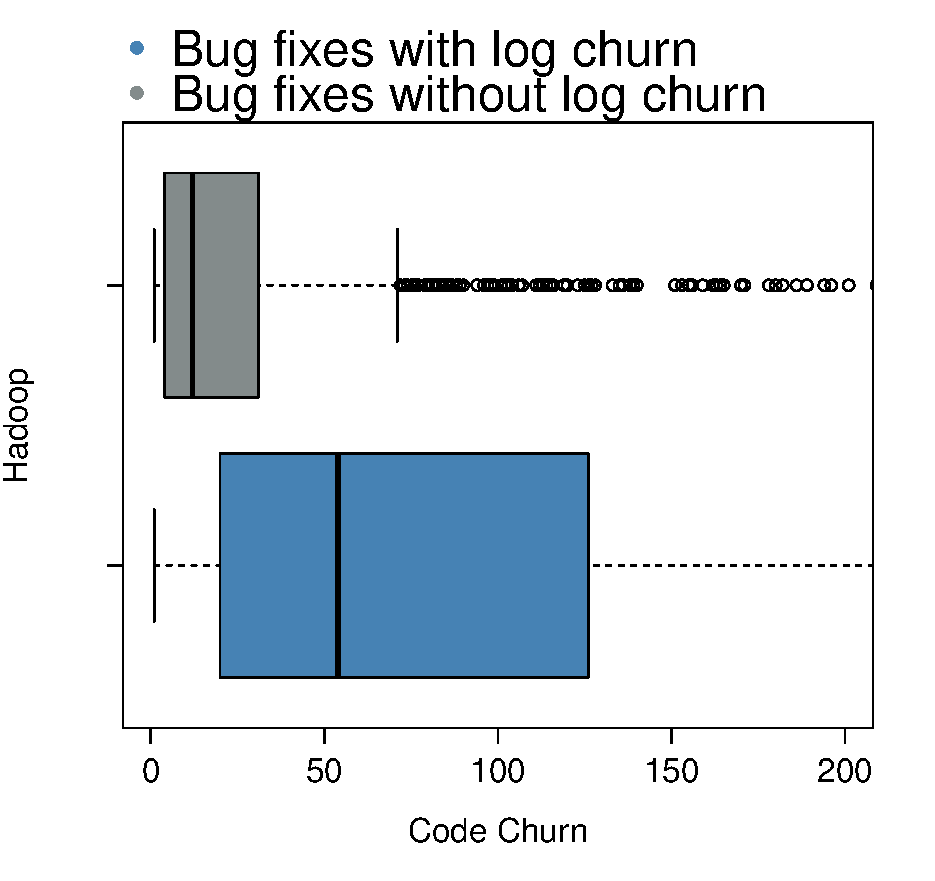
\includegraphics[width=.25\textwidth]{HadoopBoxPlot}
	\hfill
	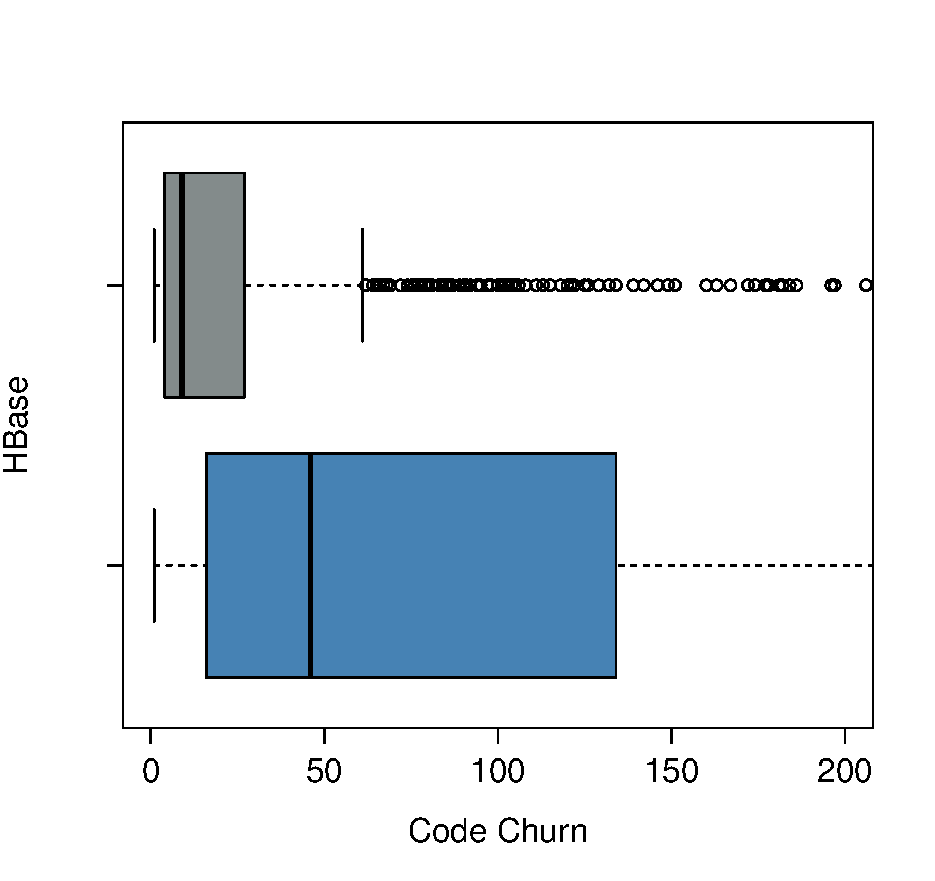
\includegraphics[width=.25\textwidth]{HBaseBoxPlot}\hfill
	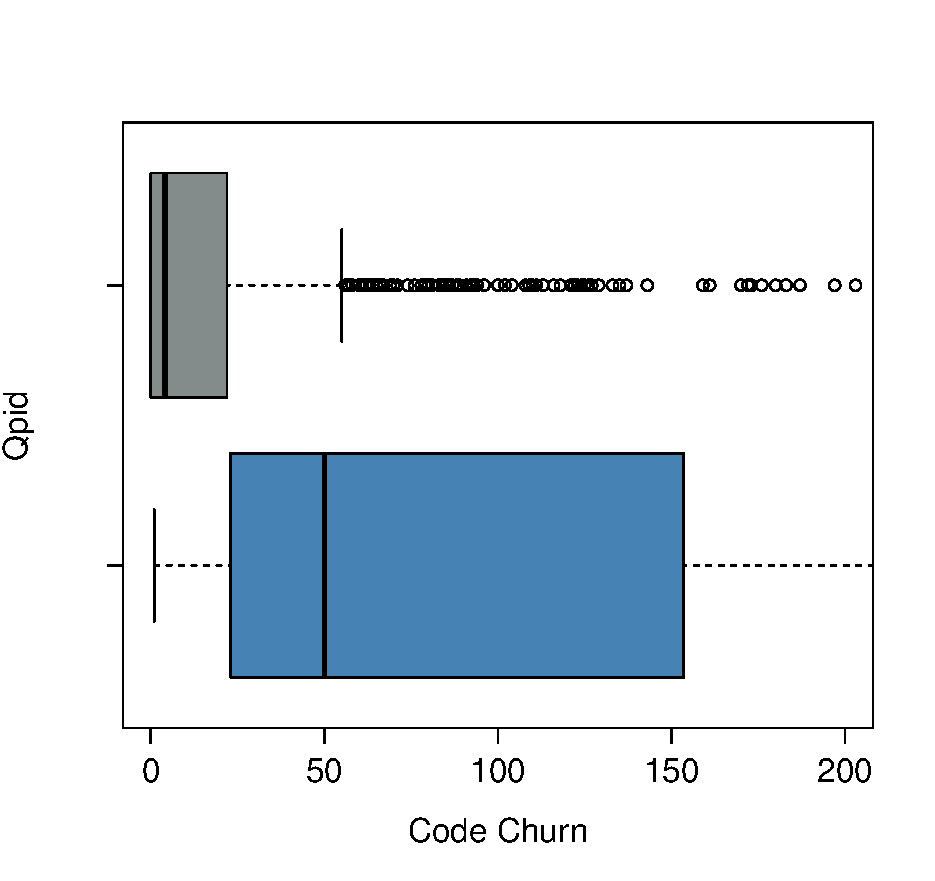
\includegraphics[width=.25\textwidth]{QpidBoxPlot}
	
	\caption{default}
	\label{fig:figure3}
	
\end{figure*}



\textbf{We found that bugs are easier to fix with logs}. After controlling the churn, we found that given two bugs of same complexity the one with log changes takes lesser time to
get resolved and needs lesser number of developers involved in the fix with less discussion. This implies that logs provide useful information for developers to discuss, diagnose and fix bugs easily. For example, logs are used in fixing issue HBASE-3074 (commit 1,005,714).
In this JIRA issue we see the very first comment is to provide additional
details in the logging message about where the connection manager
fails. When we looked at the commit, we see that the developers add
the name of the existing server which has gone stale in the logging statements. This additional data helps trace the cause of the failure and helps in the debugging process.  


%
%Because there is less developers involved in the discussion, the number of discussions posts/comments on JIRA is also less. This is because when logs are leveraged, its easier to debug the problem so resolution time is less. Developer involvement is also less because, the bug can be traced and fixed easily and long discussions about root-cause analysis is avoided. 




%This example further validates our findings
%and shows that logs are indeed very useful in the debugging process.

\hypobox{ Logs are leveraged during complex bugs and help in quicker resolution. 
	Developers leverage logging statements to fix 	complex bugs. Bug fixes with log changes are resolved quicker with fewer people and less discussions. This implies provide useful information to fix bugs.	}

%\fbox{\begin{minipage}[t]{0.9\columnwidth}%
%\textbf{Findings}: From table 4, we find all metrics have negative effect sizes and are statistically significant.
%\textbf{Implication}: 
%This implies bugs without any log churn take
%longer to be fixed, need more involvement and discussions. This shows
%that logs play a vital role in solving bug fixes. Drawing from the
%manual study done in research question two, we observed that logs
%help in locating the buggy module and when fixes are made to the module,
%developers modify the logging statements. This is cyclic process and
%hence its vital that developers log in the initial development process.%
%\end{minipage}}

\hphantom{}
%
%To validate our study we did a manual study on to understand how logs
%are actually used in the debugging process. This is explained in further
%details in the subsequent section. 


\section{Manual Study on Bug fixes}
To further understand how developers change logs during bug fixes, we conduct a manual analysis. We collected all the bug fixes with log changes for our studied systems. We selected a 5\% random sample (266 for \textsl{HBase}, 268 for \textsl{Hadoop} and 83 for \textsl{Qpid}) from all the commits. For the sampled commits, we manually examine the code changes and the corresponding JIRA issue reports to find the reasons of changing logs during bug fixes. We follow an iterative process, similar to prior research~\cite{seaman1999qualitative}, until we cannot find any new reasons. We find three reasons of changing logs during bug fixes as shown in Table~\ref{tba:LogUsage}. These three reasons may co-occur within a single commit. 

% The code changes are analyzed to identify common patters of log usage during debugging and JIRA issue reports are analyzed to understand the extent of log usage by developers.
\begin{table}[tbh]
	\protect\caption{Log change reasons during bug fix}
	\label{tba:LogUsage}	
	\begin{centering}
		\begin{tabular}{|>{\centering}p{2.5cm}|>{\centering}p{1.3cm}|>{\centering}p{1.3cm}|>{\centering}p{1.3cm}|}
			\hline 
			Projects & Hadoop & HBase & Qpid\tabularnewline
			\hline 
			\hline 
			Bug diagnosis & 157 & 175 & 49\tabularnewline
			\hline 
			Similar bugs detection & 156 & 170 & 42\tabularnewline
			\hline 
			Code quality assurance for bug fixes & 93 & 78 & 18\tabularnewline
			\hline 
		\end{tabular}
		\par\end{centering}
	
\end{table}
\begin{itemize}
	

\item \textbf{Bug diagnosis.} Developers change logs to print extra or different information into logs during the execution of the system. Such information is printed to ease bug diagnosis.
%The log changes in the category have added and deleted code prior to log changes (i.e., code block is changed). 
For example, HADOOP-2725\footnote{https://issues.apache.org/jira/browse/HADOOP-2725} is reported when users find that after copying a 100TB file across two clusters, the file sizes has a discrepancy of 6GB. However, the existing logs do not have proper format to show the size of the copied data. To help diagnose the bug, developers modify the logged variable to print the sizes of the copied data into a better format. %These log changes are committed along with bug fix, as it clarifies the log output and helps in understanding the logging context.

 %These findings are consistent with prior findings where majority of log changes are made during debugging~\cite{EMSEIAN}.

\item \textbf{Similar bugs detection.} After fixing a bug, developers may insert log into the code in order to monitor the execution of the system to detect similar bugs in the future. During the bug fixes, developers identify root-causes of the bug. After fixing the bug, developers change logs to capture the run-time event that may correspond to the root-cause of the bug, in order to identify future occurrence of a similar bug. The changed information in logs is not leveraged to fix the bug, but rather monitoring the systems for detecting a similar bug in the future. We find that logs in this category are mainly new logs being added into the system, unlike bug diagnosis which is mainly log modifications. 
%Log changes in this category have addition of new blocks (i.e., if, if-else, try-catch and exception) with higher code addition than deletion. 
For example, to fix HADOOP-2890\footnote{https://issues.apache.org/jira/browse/HADOOP-2890}, developers identify the reason behind blocks getting corrupted as an run-time exception. In the commit, we observe that the developers fix this bug and add \textsl{try catch} block with new logs to catch these exceptions. Such log will notify developers if a similar bug appears.

\item \textbf{Code quality assurance for bug fixes.} Sometime, developers need to introduce a large amounts of code to fix a bug. The introduction of bug-fixing code, may also introduce new bugs into the system. To ensure the quality of these bug fixes, developers insert new logs into the bug-fixing code. For example, in HBASE-3787\footnote{https://issues.apache.org/jira/browse/HBASE-3787}, developers encounter a non-idempotent operation (i.e., running the operation more than once produces different results) that causes an error in the application. The fix of this bug involves over 13 developers and 112 discussions over the two years. The developers add several new files and functions during the bug fix, and added logs to assure the code quality of the fix. 
\end{itemize}

\section{Limitations and Threats to Validity}

In this section, we discuss the threats to the validity to our findings.

\subsection*{External Validity}


Our case study is performed \emph{Hadoop}, \emph{HBase} and \emph{Qpid}. Even though these three studied projects have years of history and large user bases, the three studied projects are all Java based platform software. Systems in other domain may not rely on logs in bug fixes. More case studies on other software in other domains with other programming languages are needed to see whether our findings can be generalized. 


%The other limitation is projects in which logging data is less. We
%ran experiments on several other projects like Cassandra, Cayene,
%Zookeeper and Lucene. In all these projects the total number of logging
%statements were less to draw any meaningful conclusions. When we manually
%examined the data for Cassandra and Lucene we observed many custom
%logs which were not caught from pattern matching. As
%stated above its almost impossible to catch all instances of these
%custom logs in projects.


\subsection*{Internal Validity}


Our study is based on the data obtained from git and JIRA for all the studied systems. The quality of the data contained in the repositories can impact the internal validity of our study.

Our analysis of the relationship between changes to logs and bug resolution time cannot claim causal effects, as we are investigating correlations, rather than conducting impact studies. The explanative power of log churn metrics on the resolution time of bugs does not indicate that logs cause faster resolution of bugs. Instead, it indicates the possibility of a relation that should be studied in depth through user studies.


\subsection*{Construct Validity}

The heuristics to extract logging source code may not be able to extract every log in the source code. Even though the studied projects leverage logging libraries to generate logs at runtime, there still exist user-defined logs. By manually examining the source code, we believe that we extract most of the logs. %Evaluation on the coverage of our extracted logs can address this threat.

%We use keywords to identify bug fixes when the JIRA issue ID is not included in the commit messages.\ian{I thought you remove the commits without jira id!} Although such keywords are used extensively in prior research~\cite{EMSEIAN}, we may still miss identify bug fixes or branching and merging commits. 

We use Levenshtein ratio and choose a threshold to identify modifications to logs. However, such threshold may not accurately identify  modifications to logs. Further sensitivity analysis on such threshold is needed to better understand the impact of the threshold to our findings.

We build non-liner regression models using log churn metrics, to model the resolution time of bugs. However, the resolution time of bugs can be correlated to many factors other than just logs, such as the complexity of code fixes. To reduce such a possibility, we normalize the log churn metrics by code churn. However, other factors may also have an impact on the resolution time of bugs. Furthermore, as this is the first exploration (to our best knowledge) in modeling resolution time of bugs using log churn metrics, we are only interested in understanding the correlation between the two. Future studies should build more complex models, that consider other factors to study if there is any causation. 

Source code from different components of a system may have various characteristics. The importance of logs in bug fixes may vary in different components of the studied projects. More empirical studies on the use of logs in fixing bugs for different components of the systems are needed.



%

%commits which has type Branching in them and removed these
%branching commits from our data set. But we later found some of the
%commits are tagged under the category of UNKNOWN. When its under 'Unknown'
%category it was impossible to know if its branching or not. 

\section{Conclusion and Future Work}
Logs are used by developers for fixing bugs. This paper is a first attempt (to our best knowledge) to understand whether logs are changed more during bug fixes and how these changes occur. The highlights of our findings are:

\begin{itemize}
	\item We find that logs are more likely to be changed during bug fixes than non-bug fixes. In particular, we find that logs are modified more likely during bug fixes than non-bug fixes. Variables and textual information in the logs are more likely to be modified during bug fixes than non-bug fixes. 
	\item We find that logs are more likely to be changed during fixing more complex bug fixes. However, bug fixes that change logs are fixed faster, need fewer developers and have less discussion.
	\item We find that log churn metrics can complement the traditional metrics such as the number of comments and the number of developers in modeling the resolution time of bugs. 
\end{itemize} 

Our findings show that logs are changed more in bug fixes and there is a relationship between changing logs and the resolution time of bugs. Developers should allocate more effort for considering the text, the logged variables and the verbosity levels in the logs the logs are added into the source code. Hence, bugs can be fixed faster without the necessity to change logs during the fix of bugs. 


\bibliographystyle{abbrv}
\bibliography{C:/Users/Suhas/Dropbox/Logreference}


%\balancecolumns



\end{document}
